\documentclass[ 11pt]{article}
\usepackage[utf8]{inputenc}
\usepackage[a4paper,width=160mm,top=25mm,bottom=25mm]{geometry}
\usepackage{graphicx}
\usepackage{booktabs,	longtable, makecell}
\usepackage{multirow}
\usepackage{caption}
\usepackage{subcaption}
\usepackage{amsmath}
\usepackage{amsfonts}
\usepackage{bm}
\usepackage{amssymb}
\usepackage{soul}
\usepackage{array,multirow,makecell}
\newcolumntype{C}[1]{>{\centering\arraybackslash }b{#1}}

\usepackage[style = authoryear, url=false]{biblatex}
\addbibresource{Associations_and_politics.bib}
\addbibresource{Networks_Theory.bib}
\addbibresource{biblio_opinion_dynamics.bib}
\addbibresource{Lobbying.bib}
\addbibresource{additional.bib}


\title{Lobbying in the European Commission:\\ A hypergraph analysis }
\date{}
\begin{document}
\maketitle

The complex and multi-level structure of European Union institutions has led to substantial public and academic debate about their legitimacy  and democratic quality  \parencite{schmitt1999political,holzhacker2007democratic}. One of the focal point of this debate is the European Commission (EC) that is often seen as lacking electoral-based legitimacy \parencite{drake1997european,tsakatika2005claims,schmidt_europes_2020,thomas_democratic_2009}.
In view of  addressing these concerns, the Treaty on European Union has aimed to introduce a from of ``consultative legitimacy" by specifying in its article 11 that   "\textit{The European Commission shall carry out broad consultations with parties concerned in order to ensure that the Union's actions are coherent and transparent.}"  The Treaty further specifies  that these engagements with interest groups must align with specific performance criteria: accountability, transparency, efficiency, openness, and inclusiveness \parencite{schmidt_europes_2020}.  In this paper, we use a large open dataset on  meetings between European commissioners and stakeholders to investigate quantitatively whether the actual implementation of the consultation process is in line  with the principles of openness and inclusiveness put forward. Openness entails granting all parties, whether organizations or citizens, the opportunity to express their views.  Inclusiveness encourages the consideration of a diverse range of perspectives, ensuring a balance and fairness in their representation.    \\

The EC consults with stakeholders through two main channels: through written/online consultations and through face-to-face meetings. Although the  former is the most common form of consultation, the latter has been identified as a channel through which substantial influence can be exerted \parencite{heinz_hollow_1997,noah_efriedkin_social_1998,zeng_multiplex_2016,pappi_organization_1999}. Our paper studies this high influence channel through an analysis of the network of interactions between EC commission staff (commissioners, their cabinet members, and directorate generals) and stakeholders/third-parties. Notably, we investigate whether the distribution of network centrality across agents, which is standardly considered as a measure of influence in social organisations \parencite{jackson2008social}, is consistent with the principles of openness and inclusiveness. \\
%Now, the fundamental question we aim to address is whether the principles of openness and inclusiveness continue to be upheld, especially when high levels of influence are involved. 
To investigate this, we compile information on meetings held by EC representatives and build a hypergraph, where the vertices represent EC members and organizations and hyperedges involve the entities that attend meetings.  
We begin with examining the overarching structure of the network and assess the centrality of different groups, categorized by country, organization type, and sectors.
Subsequently, our analysis narrows down to companies and groups, where we compare their size to their centrality within the network, with the aim of identifying if there is a representation bias in favor of certain subgroups.  
For our research, we draw upon data from the Transparency Register of the EU and the Orbis dataset. Meeting data is accessible through the EC members' website. \\


We have gathered data on meetings conducted by commissioners, cabinet members, and directorate generals since the commencement of the current commission's term on December 1, 2019. 
These meetings are represented using a hypergraph, which we denote as $\mathcal{H}(V, E, w)$.
In this hypergraph, $V$ encompasses the set of vertices, $E$ the set of hyperedges. The weight $w_e$ is associated with each hyperedge $e$ and corresponds to the aggregated sum of occurrences of $e$ over time.
Our resulting hypergraph features $|V| = 4868$ nodes, $|E| = 13331$ edges, and a total of $\sum_e w_e = 16870$ distinct meetings. The hypergraph has a diameter of 7.
The average size of hyperedges $e$ is $2.74$ with a standard deviation of $2.05$. 
Although the number of large  hyperedges is limited, they play a crucial role in the overall connectivity of the hypergraph, as demonstrated by the substantial correlation between betweenness centrality and the size of hyperedges, which stands at $0.73$.  \\
Here are some preliminary results. We define the strength of a node $i$ as $s_i = \sum_{e: i \in e} w_e$. The distribution of strength has a fat tail. 
We compute the weight of social categories by summing the strength of nodes belonging to the corresponding social group. \\
Figure \ref{fig: s_i_vs_country} displays the total strength per country on a logarithmic scale. 
Belgium attains a notably high value, which is mainly explained by the presence of a high number of interest groups that acts at a European level and that are localized in Brussels.
Beyond the clear overall heterogeneity, non-European country such as the United States, Switzerland are notably more represented than members of the EU. 
Additionally, among EU countries, central European countries such as Latvia, Slovenia, Bulgaria, Croatia, Hungary, Romania, Luthania, Slovekia are clearly under-represented. 
\\
\begin{figure}
\centering
 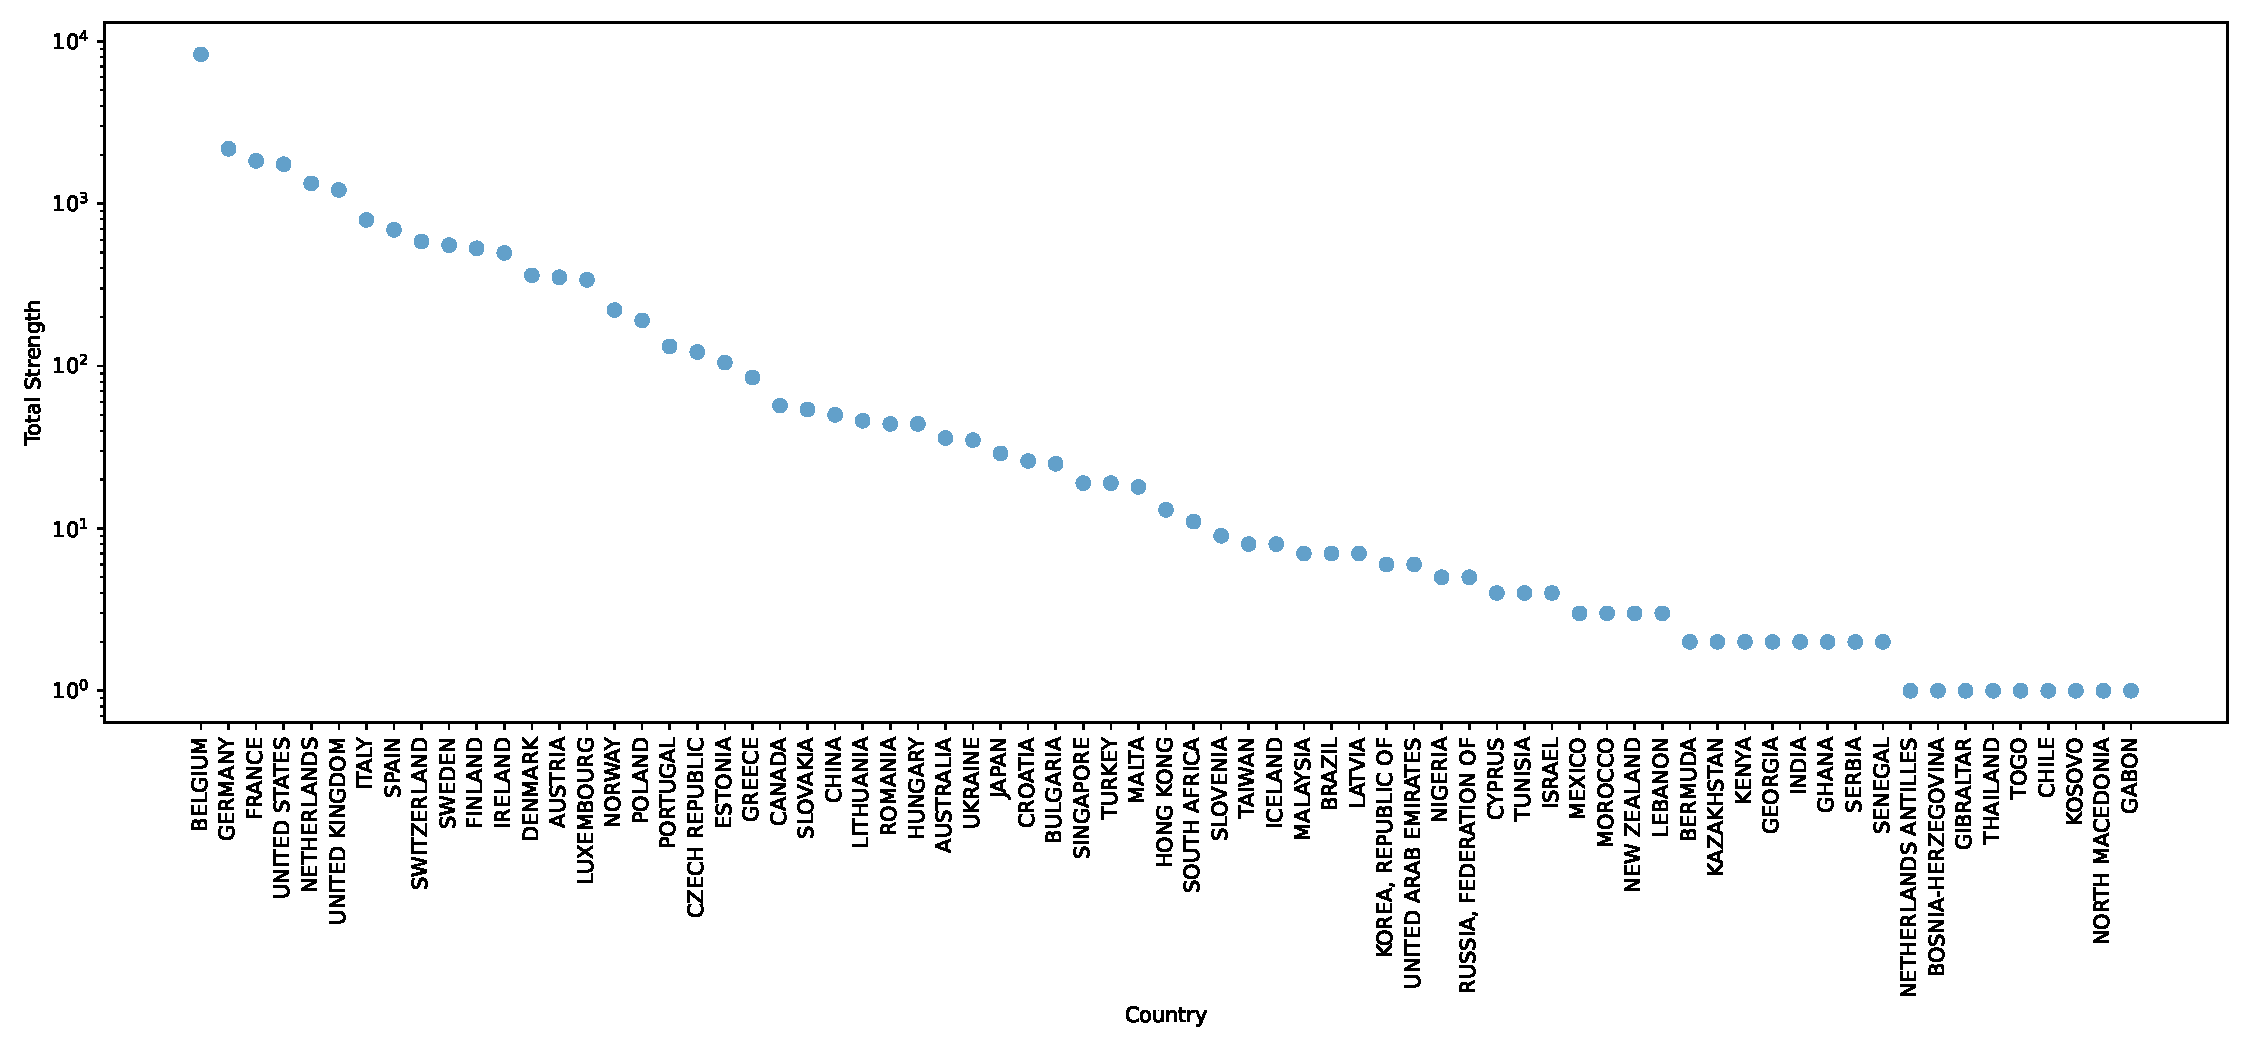
\includegraphics[scale=0.4]{/home/azaiez/Documents/Cours/These/European Commission/Programs/Figures/s_i_vs_country.pdf}
 \caption{Total strength per country. For country A, the total strength is set as $\sum_{i : i \in A } s_i$}
  \label{fig: s_i_vs_country}
\end{figure} 
In table \ref{tab: s_i_vs_cat}, we computed the strength per category of registration in the Transparency Register. Business interests represented by companies and groups as well as trade and business association are notably overrepresented.
 
 \begin{table}
 \centering
\begin{tabular}{lr}
\toprule
 & Total Strength \\
Category of registration &  \\
\midrule
Companies and groups & 7573 \\
Trade and business associations & 6015 \\
Non-governmental organisations, platforms and networks and similar & 5503 \\
Trade unions and professional associations & 1258 \\
Think tanks and research institutions & 869 \\
Professional consultancies & 607 \\
Other organisations, public or mixed entities & 524 \\
Academic institutions & 219 \\
Associations and networks of public authorities & 143 \\
Organisations representing churches and religious communities & 50 \\
\bottomrule
\end{tabular}
 \caption{Total strength per category. For category A, the total strength is set as $\sum_{i : i \in A } s_i$}\label{tab: s_i_vs_cat}
   \end{table}
   
    \newpage
    \printbibliography
   
\end{document}

@article{holzhacker2007democratic,
  title={Democratic legitimacy and the European Union},
  author={Holzhacker, Ronald},
  journal={European Integration},
  volume={29},
  number={3},
  pages={257--269},
  year={2007},
  publisher={Taylor \& Francis}
}

@article{arnold2012trust,
  title={Trust in the institutions of the European Union: A cross-country examination},
  author={Arnold, Christine and Sapir, Eliyahu and Zapryanova, Galina},
  journal={Beyond Euro-Skepticism: Understanding Attitudes Towards the EU�, European Integration Online Papers, Special Mini},
  number={2},
  year={2012}
}

@book{schmitt1999political,
  title={Political representation and legitimacy in the European Union},
  author={Schmitt, Hermann and Thomassen, Jacques},
  year={1999},
  publisher={OUP Oxford}
}


@incollection{drake1997european,
  title={The European Commission and the politics of legitimacy in the European Union},
  author={Drake, Helen},
  booktitle={At the Heart of the Union: Studies of the European Commission},
  pages={226--244},
  year={1997},
  publisher={Springer}
}

@book{jackson2008social,
  title={Social and economic networks},
  author={Jackson, Matthew O and others},
  volume={3},
  year={2008},
  publisher={Princeton university press Princeton}
}


@article{tsakatika2005claims,
  title={Claims to legitimacy: The European Commission between continuity and change},
  author={Tsakatika, Myrto},
  journal={JCMS: Journal of Common Market Studies},
  volume={43},
  number={1},
  pages={193--220},
  year={2005},
  publisher={Wiley Online Library}
}
